\section{Dijkstrův algoritmus}\label{sec:dijkstra}

Již jsme si ukázali,~že v~\emph{neohodnoceném grafu} $G=(V,E)$ umíme relativně jednoduše najít délku nejkratší cesty z~výchozího vrcholu $v_0\in V$ do ostatních vrcholů. Hrany však nemusí mít stejnou cenu. Města mohou například představovat vrcholy a~silnice mezi nimi hrany,~jejichž váhou bude délka nebo doba průjezdu.
\importantbox{Zde již nestačí počítat počet hran. Na obrázku \ref{fig:ohod_graf} je cesta $(v_0,v_1,v_2)$ levnější než přímá cesta $(v_0,v_2)$,~přestože obsahuje více hran.}
\begin{figure}[h]
    \centering
    \begin{tikzpicture}[scale=1]
    
    \node[vertex] (U1) at (0.0,0.0) {$v_0$};
    \node[vertex] (U2) at (1.5,1.5) {$v_1$};
    \node[vertex] (U3) at (3.0,0.0) {$v_2$};
    \node[vertex] (U4) at (4.5,0.0) {$v_3$};

    \draw[edge] (U1) -- node[above,midway] {$1$} (U2);
    \draw[edge] (U2) -- node[above,midway] {$1$} (U3);
    \draw[edge] (U3) -- node[above,midway] {$4$} (U4);
    \draw[edge] (U1) -- node[above,midway] {$3$} (U3);

\end{tikzpicture}

    \caption{Příklad ohodnoceného grafu.}
    \label{fig:ohod_graf}
\end{figure}
Pro kladné celočíselné váhy se nabízí převést ohodnocený graf na neohodnocený tak,~že hranu váhy $k$ nahradíme cestou o~$k$ hranách. Na nově vzniklý graf již lze aplikovat např. BFS,~které jsme popsali v~sekci \ref{sec:bfs}. Ne každý graf však musí mít \uv{malé} váhy hran. Pokud bychom vzali např. graf,~kde váhy hran jsou v~řádech tisíců,~bude pro BFS potřeba provést zbytečně mnoho práce,~neboť pro zpracování jedné ohodnocené hrany bude třeba vytvořit a~projít tisíce hran.

Jedním z~nejznámějších algoritmů pro tuto úlohu je \emph{Dijkstrův algoritmus},~který popsal v~roce 1959 nizozemský informatik \emph{Edsger W. Dijkstra}.\footnote{Dijkstrův stručný článek vyšel roku 1959; samotný algoritmus Dijkstra navrhl již roku 1956. Jeho příjmení se přibližně vyslovuje \uv{dajkstra}.} Podobně jako u~BFS a~DFS budeme postupně otevírat a~uzavírat vrcholy,~přičemž každý uzavřeme nejvýše jednou.
\importantbox{První nalezená cesta do libovolného vrcholu již nemusí být nutně nejkratší. Cestu do daného vrcholu bude třeba postupně vylepšovat.}
Zaměřme se na grafy,~jejichž váhy hran jsou nezáporné. Dijkstrův algoritmus pro graf se zápornou hranou obecně nefunguje,~a~to ani tehdy,~když graf neobsahuje záporný cyklus. Pokud navíc na cestě k~cíli leží dosažitelný cyklus se zápornou celkovou vahou,~nejkratší cesta konečné délky vůbec neexistuje. Na obrázku \ref{fig:zapor_ohod_graf} lze cyklus $(a,b,a)$ projít libovolněkrát a~každým průchodem cenu cesty snížit o~$1$. Infimum cen cest z~$s$ do $t$ je proto $-\infty$.
\begin{figure}[h]
    \centering
    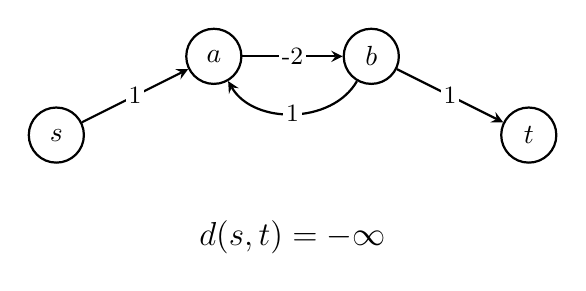
\begin{tikzpicture}[
    scale=1,
    vertex/.style={draw, circle, thick, minimum size=7mm, inner sep=0pt},
    diredge/.style={->, thick, >=stealth},
    weight/.style={fill=white, inner sep=1pt, font=\small}
]

\node[vertex] (s) at (0,0) {$s$};
\node[vertex] (a) at (2,1) {$a$};
\node[vertex] (b) at (4,1) {$b$};
\node[vertex] (t) at (6,0) {$t$};

\draw[diredge] (s) -- node[weight] {1} (a);
\draw[diredge] (a) -- node[weight] {-2} (b);
\draw[diredge] (b) to[bend left=60] node[weight] {1} (a);
\draw[diredge] (b) -- node[weight] {1} (t);

\node[align=center] at (3,-1.3) {\large $d(s,t)=-\infty$};

\end{tikzpicture}
    \caption{Graf,~kde mezi $v_0$ a~$v_4$ neexistuje (konečná) nejkratší cesta.}
    \label{fig:zapor_ohod_graf}
\end{figure}
Podobným grafům se tak chceme vyhnout,~neboť by naše úvahy pak již nemusely fungovat (cestu mezi vrcholy bychom mohli potenciálně do nekonečně vylepšovat a~algoritmus by se tak nikdy nezastavil).

V~dalších odstavcích budeme váhu hrany vedoucí z~vrcholu $u$ do vrcholu $v$ značit $\ell(u,v)$.
\begin{algorithm}
    \caption{\textsc{Dijkstra}}
    \KwIn{Nezáporně ohodnocený graf $G=(V,E)$ a~počáteční vrchol $v_0\in V$}
    \tcp{Inicializace}
    \ForEach{\textup{vrchol $v\in V$}}{
        $stav(v)\gets$ \textit{nenalezený}\\
        $D(v)\gets\infty$
    }
    $stav(v_0)\gets$ \textit{otevřený}\\
    $D(v_0)\gets 0$\\
    \While{\textup{existují otevřené vrcholy}}{
        \tcp{Kandidát na nejkratší cestu do sousedních vrcholů}
        $v\gets$ otevřený vrchol s~nejmenším $D$\\
        
        \ForEach{\textup{soused $w\in V$ vrcholu $v$}}{
            \tcp{Našli jsme lepší cestu}
            \If{$stav(w)\neq\textit{uzavřený}$ a~$D(v)+\ell(v,w)<D(w)$}{
                $D(w)\gets D(v)+\ell(v,w)$\\
                $stav(w)\gets$ \textit{otevřený}
            }
        }
        $stav(v)\gets$ \textit{uzavřený}
    }
    \KwOut{Seznam vzdáleností $D$}

\end{algorithm}
\begin{figure}[h]
    \centering
    \begin{tikzpicture}
    \node[vertex] (s) at (0,0) {$v_0$};
    \node[vertex] (a) at (2,1.4) {$a$};
    \node[vertex] (b) at (4,1.4) {$b$};
    \node[vertex] (c) at (2,-1.4) {$c$};
    \node[vertex] (d) at (4,-1.4) {$d$};
    \node[vertex] (t) at (6,0) {$v$};
    \foreach \x/\y/\w in {s/a/2,a/b/2,b/t/5,s/c/3,c/d/1,d/t/2,a/c/2,b/d/1}
        \draw[edge] (\x)--node[fill=white,inner sep=1pt]{$\w$}(\y);
    \draw[red,very thick] (s)--(c)--(d)--(t);
    \node[red] at (3,-2) {dosud nejlepší cesta};
\end{tikzpicture}

    \caption{Znázornění situace v~průběhu Dijkstrova algoritmu.}
    \label{fig:dijkstra_kratsi_cesta}
\end{figure}

\subsection{Správnost Dijkstrova algoritmu}

Nejprve je dobré si uvědomit,~proč algoritmus funguje. Hodnota $D(v)$ je vždy cenou nějaké již nalezené cesty z~$v_0$ do $v$,~a~proto nemůže být menší než skutečná nejkratší vzdálenost. Zbývá ukázat opačnou nerovnost ve chvíli,~kdy vrchol uzavíráme.

Označme skutečnou nejkratší vzdálenost vrcholu $x$ symbolem $d(x)$. Důkaz vedeme indukcí podle pořadí uzavíraných vrcholů. Předpokládejme pro spor,~že $v$ je první uzavíraný vrchol,~pro který $D(v)>d(v)$. Vezměme jednu nejkratší cestu z~$v_0$ do $v$. Na této cestě musí existovat první dosud neuzavřený vrchol $x$; jeho předchůdce $y$ už uzavřený je. Podle indukčního předpokladu platilo při uzavření $y$ rovnost $D(y)=d(y)$. Algoritmus tehdy zkontroloval hranu $(y,x)$,~a~proto nastavil
\[D(x)\leqslant d(y)+\ell(y,x)=d(x)\leqslant d(v)<D(v).\]
Využili jsme zde nezápornost hran: vzdálenost podél nejkratší cesty se směrem k~vrcholu $v$ nemůže zmenšovat. Vrchol $x$ je tedy otevřený a~má menší hodnotu $D$ než $v$. Algoritmus by proto vybral $x$,~nikoli $v$,~což je spor.
\begin{figure}[h]
    \centering
    \begin{tikzpicture}
    \node[vertex] (s) at (0,0) {$v_0$};
    \node[vertex] (y) at (2.3,0) {$y$};
    \node[vertex,draw=red] (x) at (4.6,0) {$x$};
    \node[vertex,draw=red] (v) at (7,0) {$v$};
    \draw[edge,very thick] (s)--(y)--(x)--(v);
    \draw[dashed,blue,thick,bend left=40] (s) to node[above] {nalezená cesta ceny $D(v)$} (v);
    \node[below=5mm of x] {nejkratší cesta do $v$};
\end{tikzpicture}

    \caption{Situace při výběru vrcholu $v$,~kdy $D(v)$ neodpovídá délce nejkratší cesty.}
    \label{fig:dijkstra_vyber_vrcholu}
\end{figure}

\subsection{Časová složitost Dijkstrova algoritmu}

Zbývá nám ještě analyzovat časovou složitost. Pokud se zpětně podíváme na pseudokód algoritmu,~lze si všimnout,~že podstatnou roli bude hrát vybírání vrcholu s~minimální hodnotou $D(v)$. Nabízí se tak otázka,~jak danou operaci implementovat. První variantou je hodnoty $D$ realizovat jako prostý \emph{seznam (popř. pole)}.
\begin{theorem}[Dijkstra se seznamem]
    Dijkstrův algoritmus,~kde hodnoty $D$ ukládáme do seznamu (pole),~doběhne v~čase $\bigO{n^2+m}$.
\end{theorem}
\begin{proof}
    \begin{itemize}
        \item Inicializace zabere $\bigO{n}$ (máme $n$ vrcholů).
        \item Každý vrchol uzavřeme opět nejvýše jednou,~tzn. vnější cyklus se provede $\bigO{n}$-krát.
        \item Hledání minimálního $D$ zabere v~rámci každé iterace čas $\bigO{n}$.
        \item Stejně jako u~BFS a~DFS,~i~zde každou hranu zkontroluji nejvýše dvakrát (záleží,~zda graf $G$ je orientovaný),~tzn. $\bigO{2m}=\bigO{m}$.
    \end{itemize}
    Celkově tedy máme
    \[\overbrace{\bigO{n}}^{\text{Init}}+\underbrace{\bigO{n}\cdot\bigO{n}}_{\text{Výběr minima}}+\bigO{m}=\bigO{n^2+n+m}=\bigO{n^2+m}.\]
\end{proof}
Kvadratická časová složitost není úplně zlá,~ale můžeme si ještě trochu přilepšit. Pokud si vzpomeneme na binární haldu z~oddílu \ref{sec:halda},~všimneme si v~konečném důsledku,~že při použití v~Dijkstrově algoritmu se některé operace zrychlí.
\begin{theorem}[Dijkstra s~haldou]
    Dijkstrův algoritmus,~kde hodnoty $D$ ukládáme do binární haldy,~doběhne v~čase $\bigO{(n+m)\cdot\log{n}}$.
\end{theorem}
\begin{proof}
    Inicializace trvá zase $\bigO{n}$. U~operací s~binární haldou víme,~jak dlouho potrvají (viz tabulka \ref{tab:halda_pole_operace}). Musíme si jen rozmyslet,~kdy se která operace provádí.
    \begin{itemize}
        \item Při prvním \emph{otevření} vrcholu provedeme v~haldě operaci \textsc{Insert}. Celkově vložíme nejvýše všech $n$ vrcholů,~což potrvá $\bigO{n\log n}$.
        \item Při \emph{uzavírání} vrcholu provádíme operaci \textsc{ExtractMin} (opět max. $n$-krát),~tj. $n\cdot\bigO{\log{n}}=\bigO{n\log{n}}$.
        \item Při každé další \emph{aktualizaci vzdálenosti} $D(v)$ provádíme \textsc{Decrease} (tato hodnota se nikdy nemůže zvýšit). Aktualizací je nejvýše tolik,~kolik kontrol hran,~tedy $\bigO{m}$. Dostáváme nejvýše $m\cdot\bigO{\log n}=\bigO{m\log n}$.
    \end{itemize}
    Po sečtení dostaneme
    \begin{align*}
        \bigO{n+n\log{n}+n\log{n}+m\log{n}}&=\bigO{n+2n\log{n}+m\log{n}}\\
        &=\bigO{n+n\log{n}+m\log{n}}\\
        &=\bigO{n\log{n}+m\log{n}}\\
        &=\bigO{(n+m)\cdot\log{n}}.
    \end{align*}
\end{proof}
Ačkoliv to není úplně zjevné,~výraz $(n+m)\cdot\log{n}$ roste o~dost pomaleji oproti $n^2+m$,~tedy binární haldou si skutečně pomůžeme oproti seznamu.

Závěrem uveďme,~že často nehledáme cestu do všech vrcholů,~ale pouze mezi konkrétní dvojicí. Výpočet můžeme zastavit ve chvíli,~kdy cílový vrchol vybereme jako minimum a~uzavřeme jej: tehdy už je jeho hodnota $D$ konečná. Hledání lze v~některých situacích dále urychlit,~protože Dijkstrův algoritmus může prozkoumávat i~vrcholy směřující úplně jinam než k~cíli. Na to se podíváme v~další sekci \ref{sec:astar}.
